\chapter{Identifiability and statistical visibility}\label{ch:identifiability}

An identifiability question asks whether distinct generative structures produce the same observed law. A visibility question asks how strongly those laws separate on a finite experiment. Exact nonidentification prevents recovery of the unidentified quantity from the observed law, whereas distinct laws can still be difficult to distinguish on a finite horizon. The distinction is essential here: stress memory disappears from the rate at zero feedback, yet under stronger assumptions it becomes identifiable when inhibition is active.

\section{Physical loading and the diagnostic family}

Let \(Q_i\) denote marks, let \(\Phi_s\) be a nonnegative normalized relaxation kernel, and put
\[
X(t)=X_0\Phi_s(t)+\rho\int_0^t\Phi_s(u)\,\dif u-G_s(t),
\qquad
G_s(t)=\sum_{T_i<t}g(Q_i)\Phi_s(t-T_i).
\]
The physical rate family is
\begin{equation}
\lambda_{\mathrm{phys}}(t)
=\exp\{a+bX(t)\}+nH_e(t),
\qquad
H_e(t)=\sum_{T_i<t}\kappa(Q_i)h_e(t-T_i).
\label{eq:physical-rate}
\end{equation}
Here \(\kappa\) is a unit trigger amplitude, \(\E \kappa(Q)=1\), and \(n\) is outside \(H_e\). Marks are generated from the common fresh-mark law specified for the experiment. The diagnostic experiment instead uses
\begin{equation}
\lambda_\eta(t)=B(t)e^{-\eta G_s(t)}+nH_e(t),
\qquad
B(t)=A e^{d x(t)},\qquad \eta\ge0,
\label{eq:diagnostic-rate}
\end{equation}
with the same event and mark parents supplying \(G_s\) and \(H_e\). Thus \(nH_e\) has the same unit interpretation as in \eqref{eq:physical-rate}.

The independent background \(B(t)\) in the diagnostic family is not a reparameterization of the physical loading law. In the diagnostic model, \(B(t)=A e^{d x(t)}\) is an explicitly fitted background trajectory; in the physical model, the stress response is constrained by the relaxation kernel and by the latent initial stress. This distinction is part of the inferential target, not merely a matter of notation. It is also the reason a fitted background trend cannot by itself establish earthquake-induced inhibition. Productivity is displayed in the unit convention, with its branching coefficient separate.

\section{Exact nonidentification at zero feedback}

The first nonidentification result follows directly from the multiplicative role of \(b\). If the stress sensitivity \(b=0\) while \(X_0\) and \(\rho\) remain finite, then \(bX(t)=0\) for every history. Consequently the conditional intensity is
\[
\lambda(t)=\exp(a)+nH_e(t),
\]
which contains neither \(\Phi_s\) nor \(G_s\). Different relaxation kernels can therefore imply radically different latent stress trajectories while leaving the rate and the common mark law unchanged.

\begin{proposition}[Stress-kernel nonidentification at zero feedback]
\label{prop:nonidentification}
Fix \(a\), \(n\), the trigger kernel \(h_e\), the unit-amplitude law of \(\kappa(Q)\), and the common conditional mark law. Let \(\Phi_s\) and \(\widetilde\Phi_s\) be two normalized relaxation kernels defining \eqref{eq:physical-rate} with the same finite \(X_0,\rho\) and \(b=0\). Suppose both constructions are nonexplosive. Then the two observed marked-catalogue laws agree on every finite horizon and hence on the generated infinite-horizon \(\sigma\)-field.
\end{proposition}

\begin{proof}
For either kernel the physical rate is \(\lambda_0(t)=\exp(a)+nH_e(t)\), with identical successive waiting-time hazards and fresh-mark distributions. If the common mark law has density \(p_Q\), the joint path density has the factorization
\[
\prod_{i=1}^{N}\{\lambda_0(T_i)p_Q(Q_i)\}
\exp\!\left\{-\int_0^T\lambda_0(t)\,\dif t\right\}.
\]
Every \(H_e(T_i)\) excludes event \(i\), and the stress kernel does not appear. For a general common mark measure the successive-hazard argument gives the same conclusion without a mark density. Equality on nested finite windows extends to their generated infinite-horizon sigma field.
\end{proof}

The proof uses equality of the fresh mark laws. Equality of ground intensities alone is not equality of marked laws if the conditional mark distributions differ: the same event times with different marks produce different full catalogue laws. The statement also concerns normalized relaxation kernels; it does not assert invariance to kernel-dependent changes in the trigger mechanism. The latent stress laws may be substantively different, including in their unobserved tails, even though every observed waiting time and mark has the same distribution.

In the diagnostic family the same argument applies at \(\eta=0\), holding background and triggering fixed. A shared-kernel restriction may still permit estimation of the kernel through triggering. Such estimation cannot validate the additional claim that an unobserved stress response has that same kernel.

There is a distinct singular closure as the positive stress sensitivity approaches zero. For \(b>0\), put \(p=bX_0\), \(q=b\rho\), and \(r=b\). The physical background component \(\mu_b=\exp(a+bX)\) satisfies
\[
\log\mu_b(t)=a+p\Phi_s(t)+q\int_0^t\Phi_s(u)\,\dif u-rG_s(t).
\]
Allowing \(r=0\) while \(q>0\) creates a deterministic kernel-shaped trend with no event-dependent inhibition. Reaching this closure requires \(\rho=q/r\) to diverge; retaining nonzero \(p\) also requires \(X_0=p/r\) to diverge. With fixed finite \(X_0\), therefore, \(p\to0\). The loading constraint \(\rho\ge0\) preserves \(q\ge0\). This trend-only closure and the finite-parameter \(b=0\) null are different hypotheses. A deterministic trend may identify aspects of \(\Phi_s\) through loading without identifying earthquake-induced inhibition or establishing \(h_e=-\Phi_s'\).

\section{Restricted active identification}

Nonidentification in the physical family does not mean that active inhibition is never identifiable. A deliberately restricted marked experiment can remove the zero-feedback ambiguity by exposing the nonlinear intervention term. The following statement is an idealized full-law result, not a finite-sample guarantee.

\begin{proposition}[Restricted active identification]
\label{prop:active_identification}
Consider the diagnostic family \eqref{eq:diagnostic-rate} with empty initial history, a positive continuous deterministic background \(B\), known positive continuous \(g\), and nonnegative \(\eta\). Let the known transform \(\kappa>0\) be continuous with \(\E \kappa(Q)=1\) and \(\kappa(q)\to\infty\), and let the common fresh mark law have a positive density on \([0,\infty)\). Let \(h_e\) be locally integrable at zero, continuous and positive for \(u>0\), normalized to integrate to one, and let \(\Phi_s\) be nonnegative continuous with \(\Phi_s(0)=1\). Assume all models are nonexplosive with finite mean event counts. Equality of two observed marked laws identifies \(B(t)\) on \([0,T]\), the product \(n h_e(u)\) for observed lags \(0<u<T\), and \(\eta\); if \(\eta>0\), \(\Phi_s\) is identical on \([0,T]\). For the scaled finite positive exponential-mixture family with known weights and relative rates, and \(n>0\), the mixture scale and \(n\) are also identified within that restricted family.
\end{proposition}

\begin{proof}
Before the first event \(G_s=H_e=0\), so the hazard is \(B(t)\). The distribution of the first waiting time identifies \(\int_0^tB(u)\,\dif u\), and continuity identifies \(B\) itself. Marked-law equality therefore permits comparison along a history containing one event at \(s\) with mark \(q\) and no further event before \(t\). Local integrability of \(h_e\) gives a positive no-further-event survival on each finite interval. For almost every \(s< t\) and \(q\ge0\), equality of the two hazards gives
\[
B(t)\exp\{-\eta g(q)\Phi_s(t-s)\}+n\kappa(q)h_e(t-s)
=
\widetilde B(t)\exp\{-\widetilde\eta g(q)\widetilde\Phi_s(t-s)\}
+\widetilde n\kappa(q)\widetilde h_e(t-s).
\]
Continuity extends this almost-everywhere identity to every finite \(q\) and positive observed lag. After \(B=\widetilde B\), divide by \(\kappa(q)\) and let \(q\to\infty\). The first term is bounded by \(B(t)\), while \(\kappa(q)\to\infty\); hence the normalized triggering term is identified as \(n h_e(u)=\widetilde n\widetilde h_e(u)\). Subtract this common term. The remaining background is positive on the observation window, so taking logarithms shows that \(\eta g(q)\Phi_s(u)=\widetilde\eta g(q)\widetilde\Phi_s(u)\). Dividing by the known positive \(g(q)\), and then letting \(u\downarrow0\) with \(\Phi_s(0)=1\), identifies \(\eta\). If \(\eta>0\), division by \(\eta\) identifies \(\Phi_s(u)\) throughout the observed window.

For the finite mixture \(h_e(u)=\sum_j w_j(c_je)^{-1}\exp\{-u/(c_je)\}\), the ratio \(-h_e'(0)/h_e(0)\) identifies the common scale \(e\) when the identified product \(n h_e\) is positive. Its value at zero then identifies \(n\).
\end{proof}

Several limitations are part of the result. If \(\eta=0\), the stress kernel is unidentified; if \(n=0\), the triggering scales are unidentified, even though the background may be known. The proof uses arbitrarily large marks across the full probability law. Bounded marks do not inherit this positive-identification proof: the limiting operation \(q\to\infty\) is unavailable, so a separate argument would be needed. Shared triggering may identify a trigger scale when \(\eta=0\), but it does not validate equality of the latent physical loading laws; the exact nonidentification argument remains applicable to the latent target. Unknown state-dependent mark laws, unmatched histories, random prehistory, and kernel behavior beyond the observation window are outside this restricted statement. Near-zero \(\eta\), structural identification can coexist with very weak finite-horizon separation.

\section{Instantaneous and finite-horizon visibility}

To quantify separation without invoking asymptotics, compare the diagnostic intensity \(\lambda_\eta\) with the noninhibited intensity \(\lambda_0=B+nH_e\) on the same realized history. Define
\[
p_B(t)=\frac{B(t)}{B(t)+nH_e(t)},
\qquad
\delta_\eta(t)=\frac{\lambda_0(t)-\lambda_\eta(t)}{\lambda_0(t)}
=p_B(t)\left(1-e^{-\eta G_s(t)}\right).
\]
The identity is an instantaneous comparison at fixed history. It does not simulate the different event history that inhibition would have generated, and therefore it is not a bound on the long-run causal effect of removing immigrant arrivals. Those immigrants would alter later descendants. Likewise, in a stationary uninhibited Hawkes model, \(1-n\) can be interpreted as an average immigrant fraction; that is not a pointwise identity for \(p_B\) in the varying-background inhibited family. A further masking mechanism can arise in marks: if \(\kappa(Q)\) grows faster with mark size than \(g(Q)\), then at a fixed positive lag the product \(p_BG_s\) can shrink even though the stress drop grows. Recovery time, background level, overlapping events, and kernel tails therefore matter as much as a single extreme mark.

The pointwise inequality \(0\le\delta_\eta\le p_B\) is sharp as \(\eta G_s\to\infty\) with \(p_B\) held fixed. It is useful for score geometry but is not itself a finite-horizon testing bound. The following entropy result supplies one.

\begin{proposition}[Finite-horizon visibility bound]
\label{prop:visibility}
Work on \([0,T]\) with empty history, the same bounded nonnegative deterministic background, normalized nonnegative trigger kernel, stress kernel, almost surely finite nonnegative mark transforms and fresh mark law under every \(\eta\ge0\). Assume \(\E \kappa=1\) and \(0\le n<1\). For the resulting diagnostic laws,
\begin{align}
D_{\mathrm{KL}}(P_\eta\Vert P_0)
&\le \E _\eta\int_0^T
\frac{B(t)^2}{B(t)+nH_e(t)}
\min\{\eta^2G_s(t)^2,1\}\,\dif t \\
&\le \mathcal B,\qquad \mathcal B=\int_0^T B(t)\,\dif t.
\end{align}
If also \(n>0\), \(B\le B_{\max}\), \(\kappa>0\) almost surely,
\(C_T=\int_0^T\Phi_s(u)^2/h_e(u)\,\dif u<\infty\), and
\(m=\E [g(Q)^2/\kappa(Q)]<\infty\), then
\[
D_{\mathrm{KL}}(P_\eta\Vert P_0)\le\eta^2K_T,
\qquad K_T=\frac{B_{\max}^2C_Tm\mathcal B}{n(1-n)}.
\]
Consequently every possibly randomized test \(\varphi\in[0,1]\) satisfies
\[
\E _\eta\varphi\le\E _0\varphi+
\min\{1,\eta\sqrt{K_T/2}\}.
\]
\end{proposition}

\begin{proof}
The common mark measure cancels from the likelihood ratio. Ratios in integrated expressions are set to zero where both intensities vanish; such times have no event contribution. On a fixed finite path,
\[
L_\eta=\exp\left\{\int_0^T(\lambda_0-\lambda_\eta)\dif t\right\}
\prod_i\frac{\lambda_\eta(T_i)}{\lambda_0(T_i)}
\le e^{\mathcal B}.
\]
The same bound holds after localization, so the likelihood local martingale is uniformly integrable. Subcritical Hawkes domination gives nonexplosion and \(\E _\eta N(T)\le\mathcal B/(1-n)\). These facts justify the changed law. The entropy identity is well-defined: \(\lambda_\eta\log(\lambda_0/\lambda_\eta)\le\lambda_0-\lambda_\eta\le B\) bounds the event-log expectation, and the integrated difference is also bounded by \(\mathcal B\). Substituting \(\lambda_\eta=\lambda_0(1-\delta_\eta)\) gives
\[
D_{\mathrm{KL}}(P_\eta\Vert P_0)=\E _\eta\int_0^T\lambda_0
\{(1-\delta_\eta)\log(1-\delta_\eta)+\delta_\eta\}\,\dif t.
\]
For \(0\le\delta\le1\), the bracket is at most \(\delta^2\), because their difference is \((1-\delta)(-\delta-\log(1-\delta))\ge0\). Combining this with \(1-e^{-\eta G_s}\le\min\{\eta G_s,1\}\) proves the first displayed bound. Since \(B^2/(B+nH_e)\le B\), it is at most \(\mathcal B\).

For the quadratic bound, weighted Cauchy--Schwarz gives
\[
\frac{G_s(t)^2}{H_e(t)}\le
\sum_{T_i<t}\frac{g(Q_i)^2}{\kappa(Q_i)}
\frac{\Phi_s(t-T_i)^2}{h_e(t-T_i)},
\]
with zero on an empty history. Apply this directly to
\(B^2G_s^2/(B+nH_e)\le B_{\max}^2G_s^2/(nH_e)\).
Tonelli and fresh-mark compensation bound its integrated expectation by
\[
\frac{B_{\max}^2 C_Tm}{n}\,\E _\eta N(T)\le K_T.
\]
Pinsker's inequality then bounds total variation by the square root of half the entropy, which bounds the difference in expectations of any \([0,1]\)-valued test.
\end{proof}

This is an upper bound on distinguishability with nuisances fixed; fitting cannot create information. It is not a necessary detection threshold and does not convert a feasibility calculation into a power theorem. It also does not make structural identification uniform near \(\eta=0\). The next chapter studies the likelihood and score geometry that connect these visibility statements to calibrated inference.

\section{What spatial pooling preserves}
\label{sec:regional_pooling}

The distinction between an observable statistical model and a physical mechanism also matters when regional histories are pooled. Suppose that local depletion suppresses only the background in its own region. Even with a common inhibition coefficient, adding the local intensities generally does not produce the same functional form as suppressing the total background by the summed depletion. This is a property of the exponential link, before any estimation or data analysis.

\begin{figure}[htb]
\centering
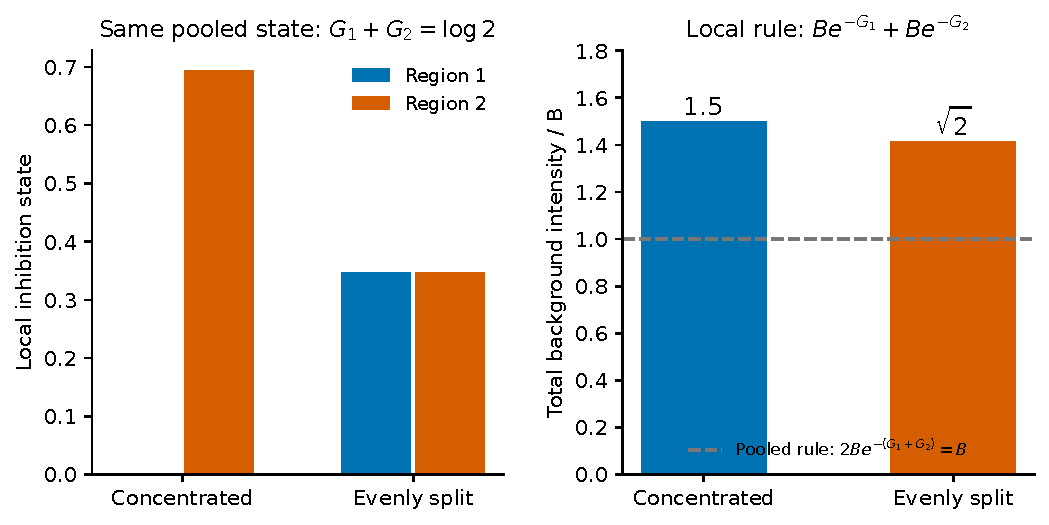
\includegraphics[width=0.85\linewidth]{pooling.pdf}
\caption{The same total depletion can have different local aggregate backgrounds. A pooled feature discards the regional allocation needed to distinguish these states. The comparison is conditional algebra, rather than an explanation of an observed predictive loss.}
\label{fig:pooling}
\end{figure}

\begin{proposition}[A conditional failure of closure under pooling]
\label{prop:regional_nonclosure}
For finitely many regions, fix $B_k\geq0$ with $B_+=\sum_kB_k>0$, nonnegative depletions $G_k$, and $\eta>0$. The local aggregate background and the pooled recipe are
\begin{equation}
 J_{\mathrm{local}}=\sum_k B_k e^{-\eta G_k},
 \qquad
 J_{\mathrm{pooled}}=B_+e^{-\eta\sum_kG_k}.
\end{equation}
The local aggregate has an effective depletion
\begin{equation}
 G_{\mathrm{eff}}=-\frac1\eta\log\left(\sum_kp_ke^{-\eta G_k}\right),
 \qquad p_k=\frac{B_k}{B_+},
 \label{eq:effective_depletion}
\end{equation}
which generally depends on the regional allocation of depletion, the background shares and $\eta$. There exist two-region backgrounds for which no function of total depletion alone, including a single rescaling of $\eta$, represents this aggregate for all regional histories. This is a failure of closure of the model class, rather than a claim that every regional configuration fails to pool.
\end{proposition}

\begin{proof}
The expression for $G_{\mathrm{eff}}$ follows by factoring $B_+$ from $J_{\mathrm{local}}$ and taking the logarithm. To show the loss of information, take two equal positive backgrounds $B$ and fix $g>0$. The histories $(G_1,G_2)=(0,g)$ and $(g/2,g/2)$ both have total depletion $g$. Their local aggregates are respectively $B(1+e^{-\eta g})$ and $2Be^{-\eta g/2}$. Their difference is
\begin{equation}
 B\bigl(1-e^{-\eta g/2}\bigr)^2>0.
\end{equation}
Every recipe using only $B_+=2B$ and $G_1+G_2=g$ gives the same value on both histories, for any common choice of its inhibition coefficient. It cannot represent both distinct local aggregates.
\end{proof}



The result permits restricted or degenerate cases in which pooling or a rescaling happens to work. It does not establish that the national recipe fails on every history, or that pooling caused the observed comparison to favour a triggering-only model. In a regional point process, adding intensities and then discarding regional labels also requires a declared filtration and a treatment of triggering across regions. Event sums assigned to spatial cells cannot supply that missing model: a joint regional likelihood includes the quiet-region compensators as well as the events. The algebra therefore motivates specifying local alternatives on a common observational target; it supplies no empirical attribution by itself.
